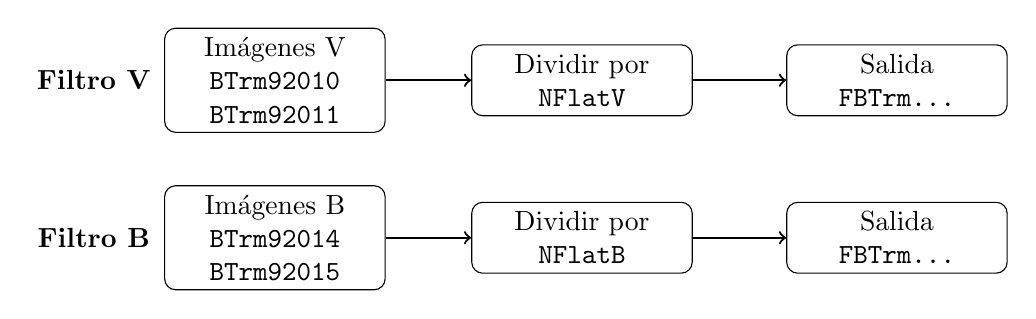
\begin{tikzpicture}[
  box/.style={draw,rounded corners,align=center,minimum width=2.8cm,minimum height=0.8cm},
  arrow/.style={->,thick}
]
  \node[font=\bfseries] at (0,1.8) {Filtro V};
  \node[box] (vscience) at (2.3,1.8) {Imágenes V\\\texttt{BTrm92010}\\\texttt{BTrm92011}};
  \node[box] (vflat) at (6.2,1.8) {Dividir por\\\texttt{NFlatV}};
  \node[box] (vout) at (10.2,1.8) {Salida\\\texttt{FBTrm...}};
  \draw[arrow] (vscience) -- (vflat);
  \draw[arrow] (vflat) -- (vout);
  \node[font=\bfseries] at (0,-0.2) {Filtro B};
  \node[box] (bscience) at (2.3,-0.2) {Imágenes B\\\texttt{BTrm92014}\\\texttt{BTrm92015}};
  \node[box] (bflat) at (6.2,-0.2) {Dividir por\\\texttt{NFlatB}};
  \node[box] (bout) at (10.2,-0.2) {Salida\\\texttt{FBTrm...}};
  \draw[arrow] (bscience) -- (bflat);
  \draw[arrow] (bflat) -- (bout);
\end{tikzpicture}